\documentclass[10pt,a4paper]{article}
\usepackage[latin1]{inputenc}
\usepackage{amsmath}
\usepackage{amsfonts}
\usepackage{amssymb}
\usepackage{graphicx}
\usepackage{hyperref}
\usepackage{float}
\begin{document}
	\title{Usage Modelling\\scalability iobserve-analysis}
	\date{}
	\maketitle
	
	\section{General}
	\textbf{Code:} \url{https://github.com/Nicolas-Boltz/iobserve-analysis-JSS-2020/tree/scalability-usability-1}\\
	\textbf{Experiment data and results:} \url{https://github.com/research-iobserve/iobserve-architectural-runtime-models-JSS-2020/tree/master/scalability_experiment}
	
	\section{Set ups:}
	For the experiment we repeatedly increase the number of accesses to the modelled system by a factor of 10, starting with 1.\\
	The increased number of accesses is reflected in the model by an increased number of monitoring entries.
	A model with a particular number of monitoring entries is called a \emph{model configuration}.
	A \emph{model configuration} can be executed by iobserve-analysis.\\
	A single execution of each model configuration from 1 to 100000 is called one \emph{run}.
	A total of 10 \emph{runs} were made for each experiment set up (equal\_events\_x\_users and x\_different\_events\_one\_user). 
	The median is taken from the values of the 10 resulting data sets of each executed \emph{model configuration}.\\
	One dataset contains the total duration of each of the filters TPreprocess and TRuntimeUpdate. 
	The total duration of a filter is gathered by \emph{calculating the sum} of the time required for each \emph{iteration} through the filter.
	The TPreprocess filter is iterated 100 times for a model configuration with 100 monitoring entries.
	The TRuntimeUpdate filter is iterated only once for each model configuration.
	
	\subsection{equal\_events\_x\_users:}
	The same call executed from X users successively. The executed call has the following signature:\\ \emph{org.cocome.cloud.logic.webservice.cashdeskline.cashdesk.CashDesk.startSale(java.lang.String,long)}
	
	\subsection{x\_different\_events\_one\_user:}
	A single user executing X calls successively. The experiment data is made up of randomly created sequences of calls taken from the CoCoMe case study, which have a direct mapping from monitoring data to the PCM model instance. The call signatures are the following:
	\emph{{\tiny
			\begin{itemize}
				\item org.cocome.cloud.logic.webservice.cashdeskline.cashdesk.barcodescanner.BarcodeScanner.sendProductBarcode(java.lang.String,long,long)
				\item org.cocome.cloud.logic.webservice.cashdeskline.cashdesk.CashDesk.startSale(java.lang.String,long)
				\item org.cocome.cloud.logic.webservice.cashdeskline.cashdesk.CashDesk.selectPaymentMode(java.lang.String,long,java.lang.String)
				\item org.cocome.cloud.logic.webservice.cashdeskline.cashdesk.CashDesk.finishSale(java.lang.String,long)
				\item org.cocome.cloud.logic.webservice.store.StoreManager.createStockItem(long,org.cocome.tradingsystem.inventory.application.store.ProductWithStockItemTO)
				\item org.cocome.tradingsystem.inventory.application.store.StoreServer.getProductWithStockItem(long,long)
				\item org.cocome.tradingsystem.inventory.application.store.StoreServer.getStore(long)
				\item org.cocome.tradingsystem.inventory.data.enterprise.StoreEnterpriseQueryProvider.queryEnterpriseByName(java.lang.String)
				\item org.cocome.tradingsystem.inventory.data.enterprise.TradingEnterprise.initTradingEnterprise()
				\item org.cocome.tradingsystem.inventory.data.store.EnterpriseStoreQueryProvider.queryStockItem(long,long)
				\item org.cocome.tradingsystem.inventory.data.store.EnterpriseStoreQueryProvider.queryStoreById(long)
				\item org.cocome.tradingsystem.inventory.data.store.Store.initStore()
				\item org.cocome.tradingsystem.inventory.data.store.StoreDatatypesFactory.fillStoreWithEnterpriseTO(org.cocome.tradingsystem.inventory.data.store.IStore)
	\end{itemize}}}
	Due to the very limited amount of different calls and random creation of call sequences, some successive sections may be identical, or may only be made up of the same successive call, resulting in loops and branches in the created UsageModel.
	
	\section{Key}
	\begin{itemize}
		\item $n$: number of entry call events; \vspace{-0.25cm}
		\item $c$: length of class signature in monitoring data; \vspace{-0.25cm}
		\item $o$: length of operation signature in monitoring data; \vspace{-0.25cm}

		\item $s$: number of user sessions; \vspace{-0,25cm}
		\item $m$: number of distinct operation signatures; \vspace{-0,25cm}
		\item $k$: number of clusters; \vspace{-0,25cm}
		\item $b$: number of branch transitions; \vspace{-0,25cm}
		\item $l$: number of loops; \vspace{-0,25cm}
		\item $e_s$: number of elements in the largest user session; \vspace{-0,25cm}
		\item $e_b$: number of elements in the largest branch transition; \vspace{-0,25cm}
		\item $e_l$: number of elements in the largest loop;
	\end{itemize}
	
	\section{TPreprocess}
	The TPreprocess filter is an abstract superordinate filter, which preprocesses the incoming monitoring data. It is made up of two connected sub-filters:
	
	\paragraph{TEntryCall}
	The monitoring data regarded by this evaluation setups is made up of three types of records. Each call starts with a TraceMetadata record, followed by a BeforeOperationObjectEvent and a corresponding AfterOperationObjectEvent. Together, these three records represent a single call from one user session. Records that are related, because they are from the same user session carry an identical session-id and call id. TEntryCall filters and maps these related records, to recreate calls which are present in the monitoring data. Once an AfterOperationObjectEvent is mapped to a previously processed BeforeOperationObjectEvent, an EntryCallEvent representing the call is forwarded to TEntryCallSequence. This is necessary, as in normal monitoring data it would be possible, that there is an arbitrary amount of records from other sessions between three related ones.\\
	TEntryCall only operates on HashMaps, which results in a time complexity of $\mathbf{O(1)}$
	
	\paragraph{TEntryCallSequence}
	While TEntryCall recreates calls, TEntryCallSequence maps the incoming EntryCallEvents according to their session-id, recreating user sessions. While mapping, all sessions that exceed a certain size are collected and forwarded. \\
	Only events that have a direct mapping to a PCM entity can be considered in the further process. To ensure this, the CorrespondenceModel is used to check if a correspondence exists for each incoming EntryCallEvent. This operation relies on parsing the class and operation signatures of the EntryCallEvent two times, which results in a time complexity of $\mathbf{O(2 * c + 2 * o)}$, for the first occurrence of each call. For the following occurrences of similar calls, with equal class and operation signature, the time complexity drops to $\mathbf{O(c + o)}$. This is due to correspondences being mapped in a HashMap once they occur, removing the need to parse the class and operation signature a second time.
	
	\paragraph{Combined}
	Combining TEntryCall and TEntryCallSequence results in a big O notation time complexity of $O(c + o)$, for single run of TPreprocess. In each of the evaluation setups, the TPreprocess filter is called $n$ times, where n is the number of monitored calls in the monitoring data. As $c$ and $o$ stay roughly the same size, $n$ grows. This is why $c$ and $o$ can be regarded as fixed values, for combined time complexity.\\
	This results in a time complexity of $n * O((c + o)) = n * O(1) \rightarrow \mathbf{O(n)}$
	
	\subsection{equal\_events\_x\_users:}
	\begin{figure}[H]
		\centering
		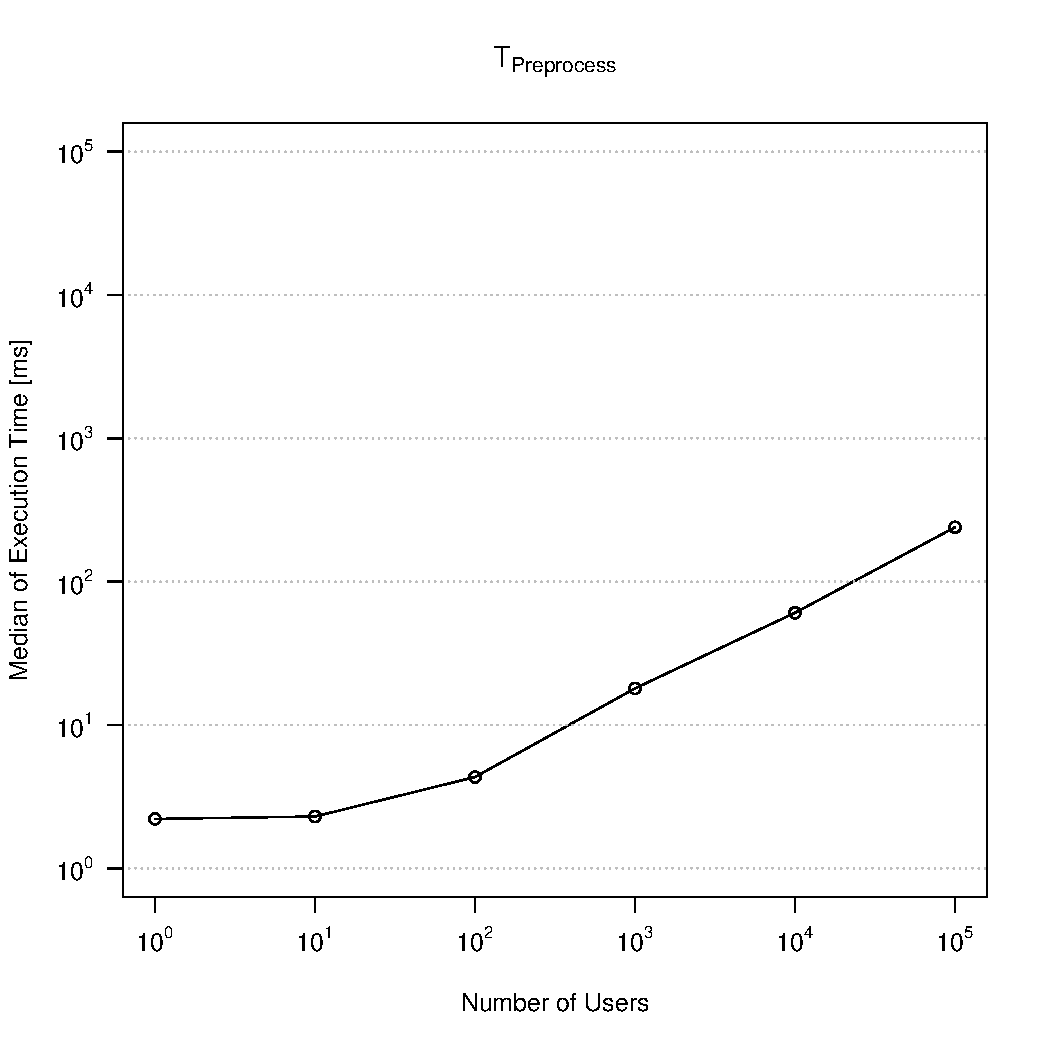
\includegraphics[scale=0.7]{graphics/TPreprocess_median_equal_events.pdf}
	\end{figure}
	For this experiment set up $\mathbf{c}$ and $\mathbf{o}$ have a fixed size, while $n$ grows linearly. This results in an complexity of $\mathbf{O(n)}$.
	
	\subsection{x\_different\_events\_one\_user:}
	\begin{figure}[H]
		\centering
		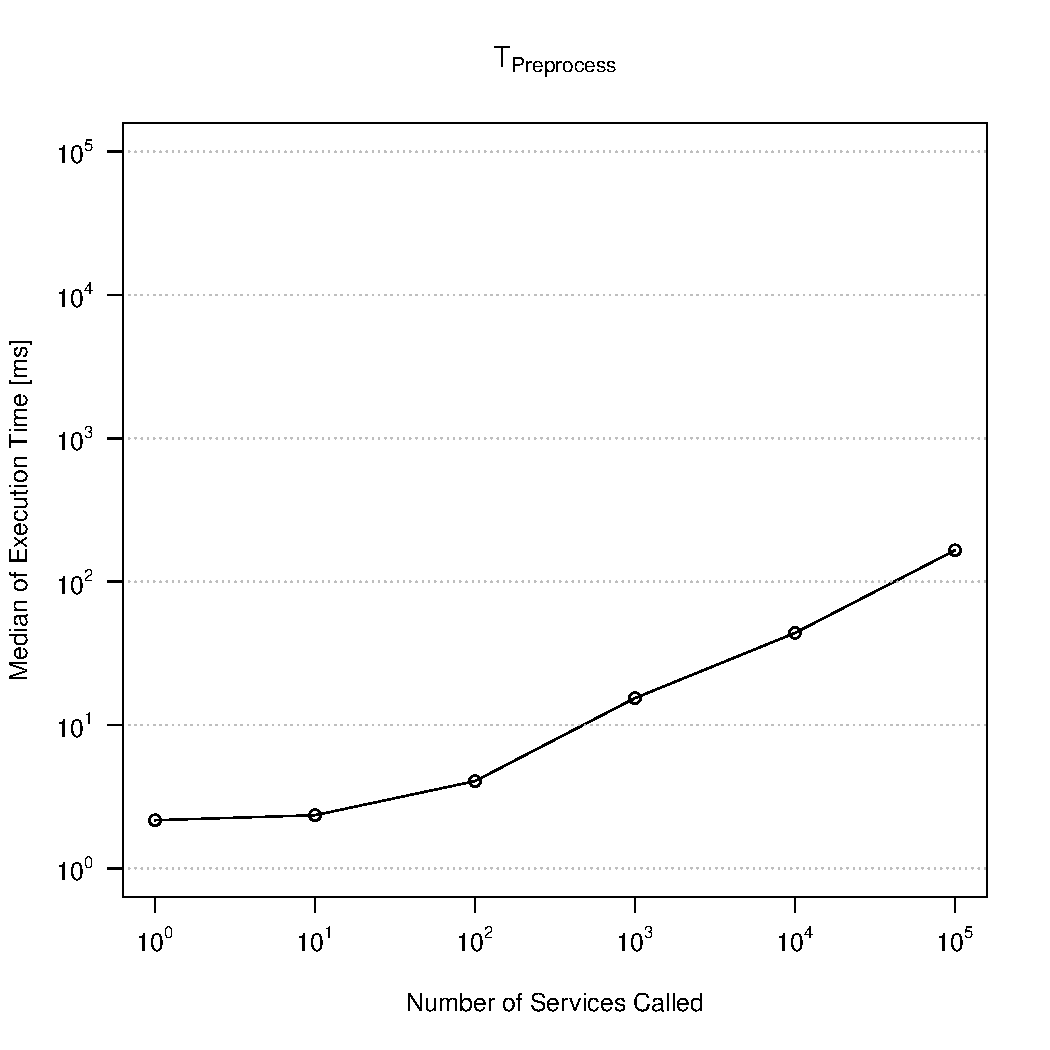
\includegraphics[scale=0.7]{graphics/TPreprocess_median_different_events.pdf}
	\end{figure}
	For this experiment set up $\mathbf{c}$ and $\mathbf{o}$ vary, while $\mathbf{n}$ grows linearly. This overall still results in a complexity of $O(n * (c + o))$. As in this experiment there are only 13 different class/operation pairs available, $c$ and $o$ can be treated like fixed values, which reduces the time complexity to $\mathbf{O(n)}$.
	\newpage
	\section{TRuntimeUpdate (TEntryEventSequence):}
	This filter loads the PCM UsageModel, uses the incoming set of user sessions to do a UserBehaviourTransformation, and writes the resulting PCM UsageModel to the disk. As times for loading and writing may vary depending on the underlying system and current use of the disk, only the UserBehaviourTransformation is regarded by this evaluation.\\
	\\
	Unlike the TPreprocess filter, which is called multiple times, the TRuntimeUpdate filter is only called \textbf{once} for each run of a scaling step ($10^0$ / $10^1$ / $10^2$ / $10^3$ / $10^4$ / $10^5$).\\
	\\
	For worst case time complexity $m$ and $k$ can be treated as constants, as they do not scale with the other variables. The maximum amount of services provided by the system $m$ usually reaches a plateau at 1000 and the amount of clusters $k$ does not exceed two digit values.

	\subsection{Breakdown of user behaviour transformation}
	The time complexity of the usage behaviour transformation is made up of the following parts:\\
	\\
    $T_{UserGroupDetection}$ identifies the distinct calls within the user sessions and then clusters the user sessions into user groups using the X-Means clustering algorithm. After clustering, it sets the workload intensity of each user group. Depending on how iobserve-analysis is set up, this is done by either calculating the number of concurrent users or the inter-arrival time of users from the user group.\\
    This results in worst-case time complexity of $O(s^{2}*e_s)$ for $T_{UserGroupDetection}$.\\
%	Alternative:
%	For the clustering of user groups first a list of distinct operation signatures is extracted from the received EntryCallSequenceModel. Then the UserSessions are transformed to a model representing counts of distinct calls of the UserSession. This model is then clustered using the xMeansClustering. After clustering, each resulting cluster is transformed to a individual EntryCallSequenceModel.\\
%	Adding these complexities results in a complexity of\\
%$O(s*e_s + s + s^2*e_s + m*n + m + 2*n*k + 5*n*k*m) \Rightarrow O(s^2 * e_s + s * e_s + s * (m+k) + n*k*m) \Rightarrow O(s^2 * e_s + n*k*m) \Rightarrow O(s^2 * e_s + n) \Rightarrow O(s^2 * e_s)$.
	\\
	For the users sessions of each user group $T_{BranchDetection}$ creates a tree structure by aggregating the contained entry calls, identifies the transition probability for each branch transition and then merges branch transitions and removes redundant branch transitions.\\
	This results in worst case time complexity of $O(slog(s) + s*e_s*b*log(b) + b^2*e_b)$.\\
	As $b^2 > blog(b)$ and $e_s \geq e_b$, due to all entry calls of a user session either being exactly represented by a single, or split into multiple branch transitions.\\
	$\Rightarrow O(slog(s) + s*e_s*b^2 + b^2*e_s) \Rightarrow O(s*log(s) + s*e_s*b^2)$.\\
%	Alternative:
%	For each created EntryCallSequenceModel, a tree structure called branch model is created, by aggregating the contained EntryCalls. Iterating over the tree, the likelihood of occurrence for each branch is calculated. After that the branch model is compacted, by combining branches with equal ends, removing any unnecessary redundant branch behaviour.\\
%$O(k * (s*log(s) + s*e_s*b*log(b) + s*e_s*b + 2*b^2*e_b + b^2)) \Rightarrow O(s*log(s) + s*e_s*b*log(b) + b^2*e_b)$\\
%As $b^2 > b*log(b)$ and $e_s \geq e_b$, due to all elements of a session either being exactly represented by, or split into multiple branch transitions.\\
%$\Rightarrow O(s*log(s) + s*e_s*b^2 + b^2*e_s) \Rightarrow O(s*log(s) + s*e_s*b^2)$.
	\\
	$T_{LoopDetection}$ traverses the tree structure recursively for each branch transition to identify loops. This has a time complexity of $O(b*e_b^{3} + b*e_b^{2}*\frac{e_b}{e_l} + b*e_l*l)$.\\
	As all elements of a branch transition could be in one big loop, it can be assumed that $e_l \leq e_b$, for worst case time complexity. Which results in $O(b*e_b^{3} + b*e_b^{2} + b*e_b*l) \Rightarrow O(b*e_b^{3} + b*e_b*l)$\\
	\\
	$T_{ArchitecturalModelUpdate}$ iterates the tree structure to create the elements of the architectural model.\\
	This shows a worst case time complexity of $O(b*(e_b + e_l))$.
	
	\paragraph{Combined:}
	Adding and reducing the time complexities of the four parts results in a complexity of $O(s^2*e_s + s*e_s*b^2 + b*e_b^{3} + b*e_b*l + b*(e_b + e_l))$. Appling the assumptions made for $T_{BranchDetection}$ and $T_{LoopDetection}$ results in a combined worst case complexity of $\mathbf{O(s^2*e_s + s*e_s*b^2 + b*e_s^{3} + b*e_s*l)}$.
	
	\subsection{equal\_events\_x\_users:}
	\begin{figure}[H]
		\centering
		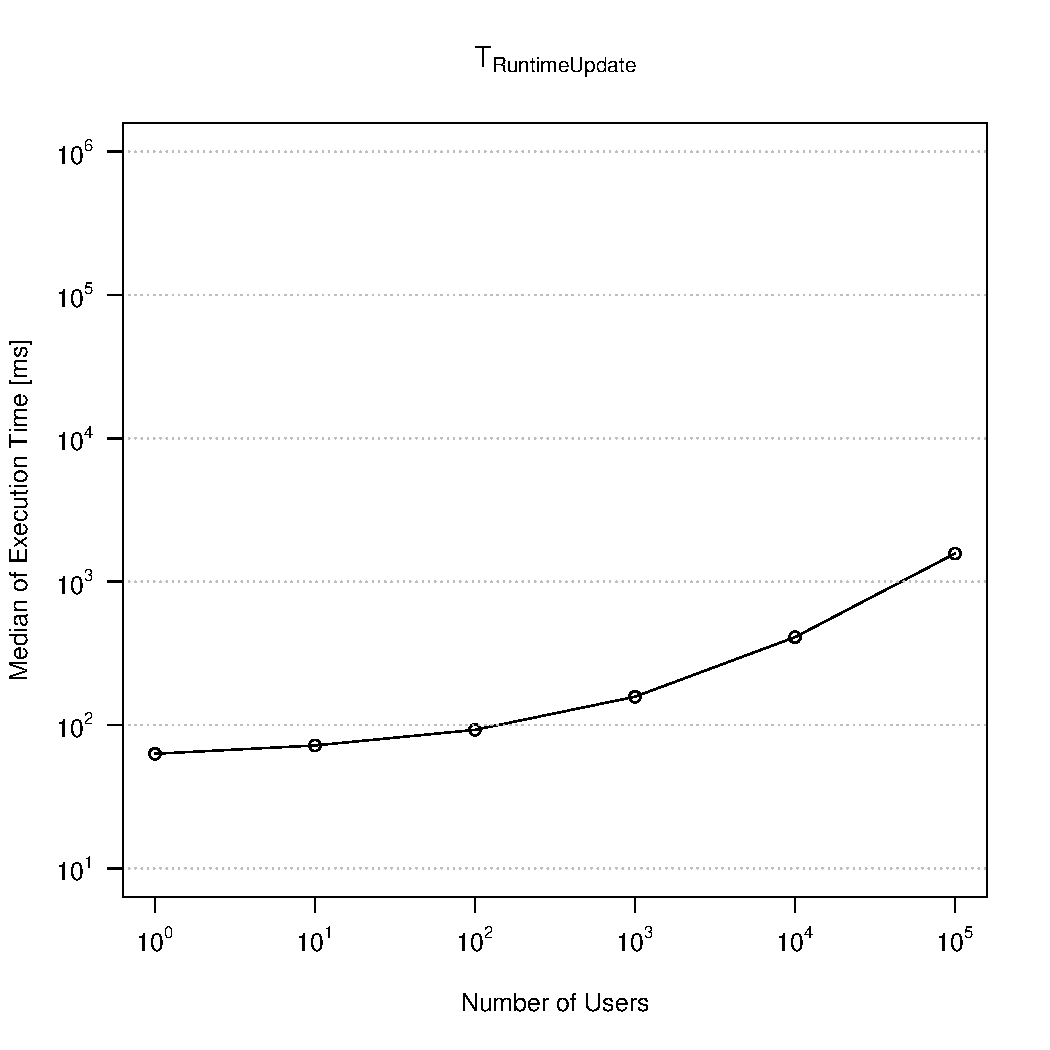
\includegraphics[scale=0.7]{graphics/TRuntimeUpdate_median_equal_events.pdf}
	\end{figure}
	For this experiment set up $\mathbf{e_s = 1, m = 1, k = 1, b = 1, e_b = 1, l = 0, e_l = 0}$, while $\mathbf{s}$ grows logarithmically by a factor of $10$ ($10^0$ / $10^1$ / $10^2$ / $10^3$ / $10^4$ / $10^5$). Applying this to the general time complexities from above results in the following complexities:\\
	Clustering: $\mathbf{O(s^2)}$\\
	Branching: $O(s * log(s) + s) \Rightarrow \mathbf{O(s * log(s))}$\\
	Loop detection: $\mathbf{O(1)}$\\
	Model build: $\mathbf{O(1)}$\\
	\\
	Combined: $O(s^2 + s * log(s)) \Rightarrow \mathbf{O(s^2)}$\\
	
	\subsection{x\_different\_events\_one\_user:}
	\begin{figure}[H]
		\centering
		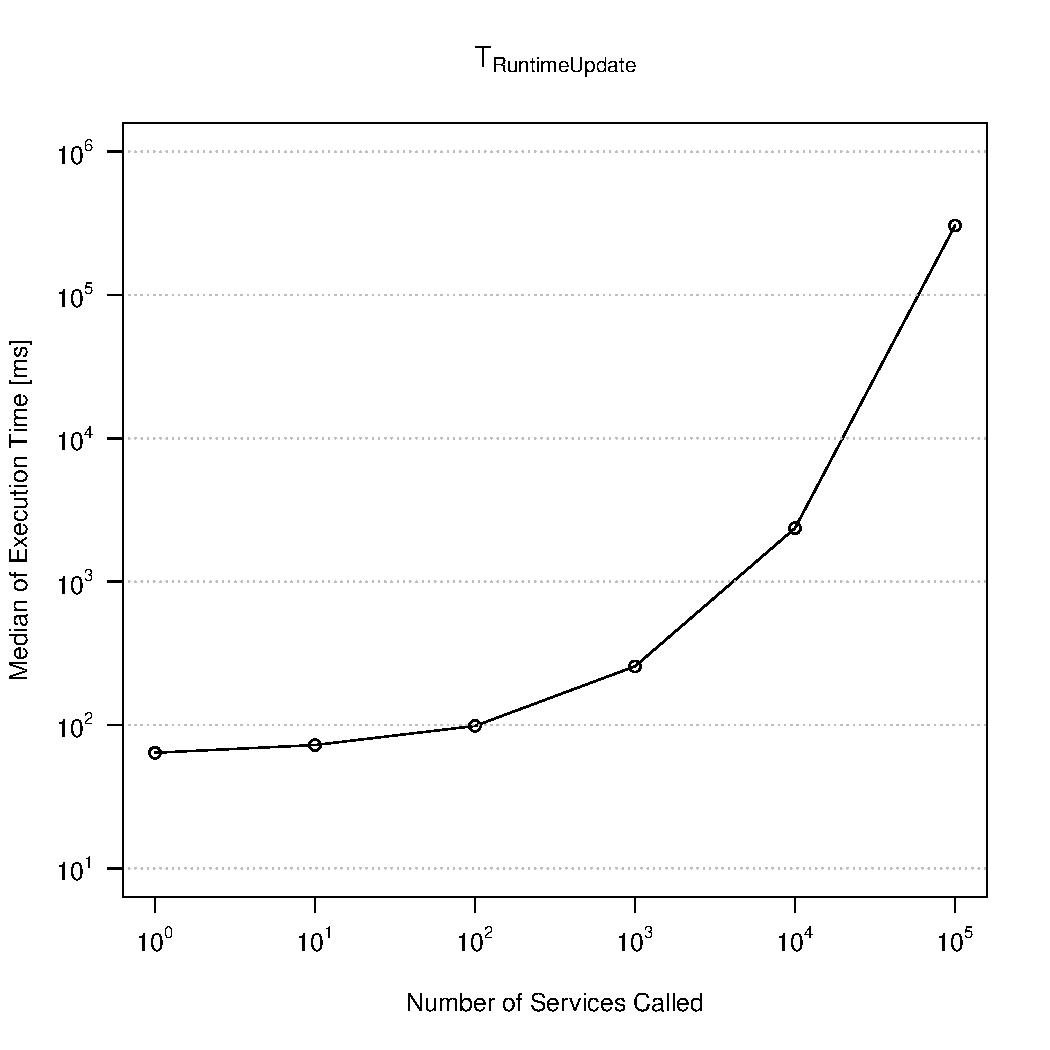
\includegraphics[scale=0.7]{graphics/TRuntimeUpdate_median_different_events.pdf}
	\end{figure}
	For this experiment set up $\mathbf{s = 1, m = 13, k = 1, b = 1}$ and $\mathbf{e_l}$ is fixed, while $\mathbf{e_s}$ and $\mathbf{e_b}$ grow logarithmically by a factor of $10$ ($10^0$ / $10^1$ / $10^2$ / $10^3$ / $10^4$ / $10^5$). The data used for running this experiment is generated by randomly as described in the experiment set ups. As there are only 13 calls, it is possible for loops to be generated. As the amount, or size of loops does not scale proportionally with the experiment size, $\mathbf{l}$ and $\mathbf{e_l}$ can be treated as a fixed constant. Applying this to the general time complexities from above results in the following complexities:\\
	Clustering: $\mathbf{O(e_s)}$\\
	Branching: $\mathbf{O(e_s)}$\\
	Loop detection: $O(e_b^3) \Rightarrow \mathbf{O(e_s^3)}$\\
	Model build: $O(e_b) \Rightarrow \mathbf{O(e_s)}$\\
	\\
	Combined: $O(e_s^3 + 3*e_s) \Rightarrow \mathbf{O(e_s^3)}$\\
	\\
	The loop detection takes up more than 90\% of the required time. This mostly corresponds to its complexity, when compared to the complexity of the other steps. Still, looking at the logging data, the clustering and branching are much lower than they should be compared to the complexity statements above. It is possible that for this one-sided scenario, with only one big user session, the branching (and also clustering) algorithm can skip most of the time consuming steps, which is not considered in the big O notation.
\end{document}